
\documentclass{standalone}
\usepackage{xcolor}
\usepackage{pgfplots}
\pgfplotsset{compat=1.18}

\begin{document}

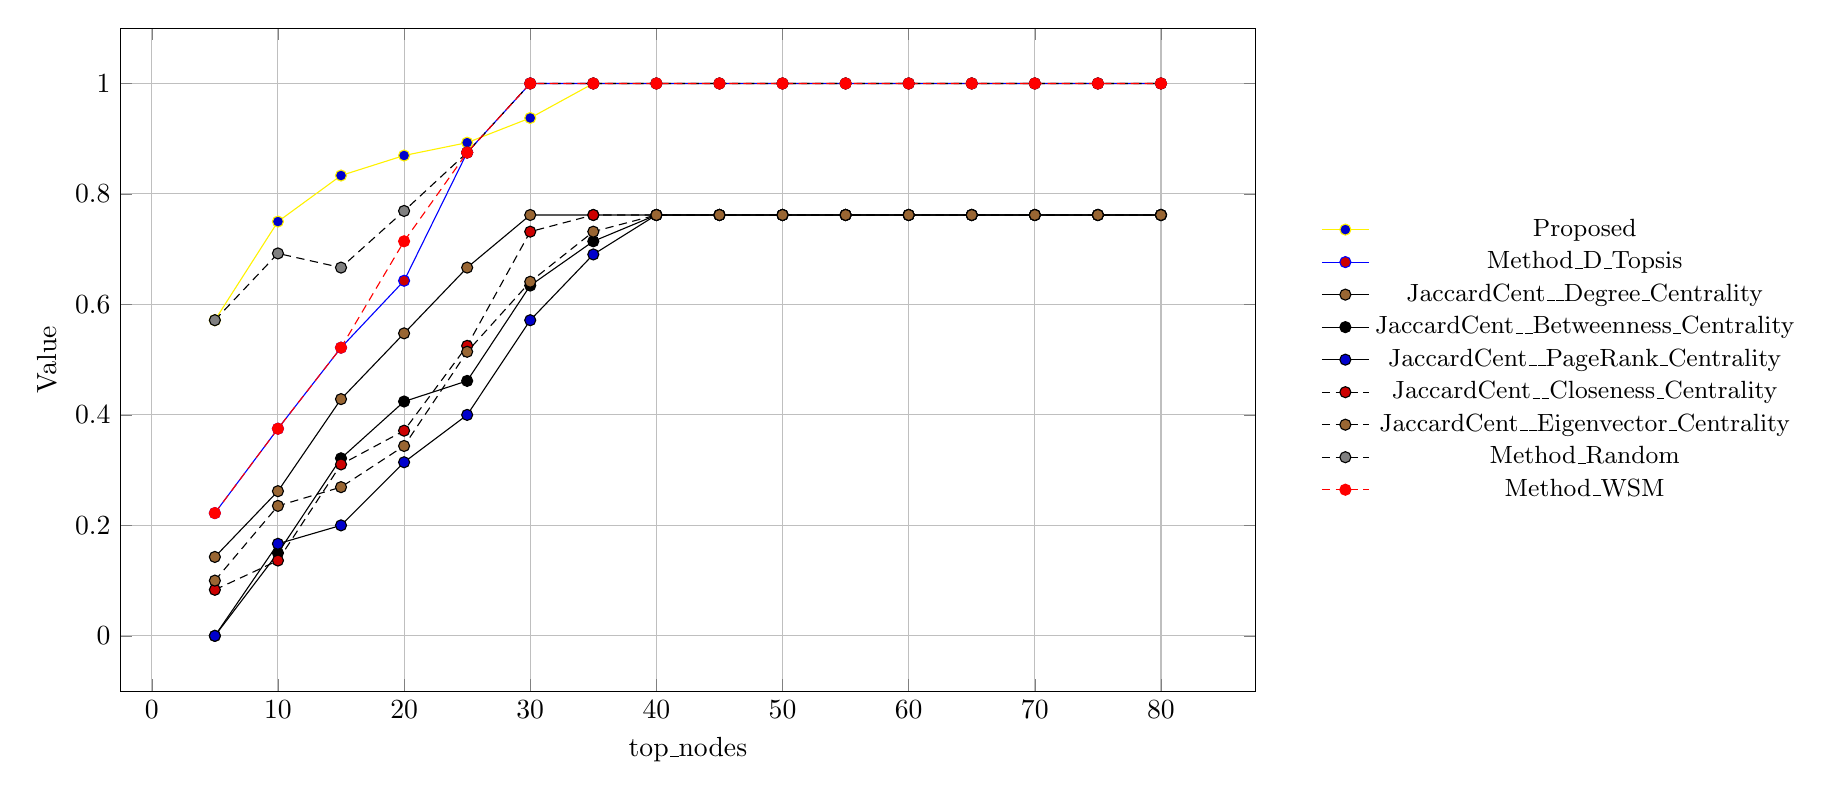
\begin{tikzpicture}
\begin{axis}[
    width=16cm,
    height=10cm,
    xlabel={top\_nodes},
    ylabel={Value},
    grid=major,
    legend style={
        at={(1.05,0.5)},
        anchor=west,
        font=\small,
        draw=none,
        cells={align=left},
    },
]
% Proposed
\addplot+[color=yellow, mark=*] coordinates {
(5.0,0.5714285714285714) (10.0,0.75) (15.0,0.8333333333333334) (20.0,0.8695652173913043) (25.0,0.8928571428571429) (30.0,0.9375) (35.0,1.0) (40.0,1.0) (45.0,1.0) (50.0,1.0) (55.0,1.0) (60.0,1.0) (65.0,1.0) (70.0,1.0) (75.0,1.0) (80.0,1.0) };
\addlegendentry{Proposed}

% Method\_D\_Topsis
\addplot+[color=blue, mark=*] coordinates {
(5.0,0.2222222222222222) (10.0,0.375) (15.0,0.5217391304347826) (20.0,0.6428571428571429) (25.0,0.875) (30.0,1.0) (35.0,1.0) (40.0,1.0) (45.0,1.0) (50.0,1.0) (55.0,1.0) (60.0,1.0) (65.0,1.0) (70.0,1.0) (75.0,1.0) (80.0,1.0) };
\addlegendentry{Method\_D\_Topsis}

% JaccardCent\_\_Degree\_Centrality
\addplot+[color=black, mark=*] coordinates {
(5.0,0.1428571428571428) (10.0,0.2619047619047619) (15.0,0.4285714285714285) (20.0,0.5476190476190477) (25.0,0.6666666666666666) (30.0,0.7619047619047619) (35.0,0.7619047619047619) (40.0,0.7619047619047619) (45.0,0.7619047619047619) (50.0,0.7619047619047619) (55.0,0.7619047619047619) (60.0,0.7619047619047619) (65.0,0.7619047619047619) (70.0,0.7619047619047619) (75.0,0.7619047619047619) (80.0,0.7619047619047619) };
\addlegendentry{JaccardCent\_\_Degree\_Centrality}

% JaccardCent\_\_Betweenness\_Centrality
\addplot+[color=black, mark=*] coordinates {
(5.0,0.0) (10.0,0.15) (15.0,0.3214285714285714) (20.0,0.4242424242424242) (25.0,0.4615384615384615) (30.0,0.6341463414634146) (35.0,0.7142857142857143) (40.0,0.7619047619047619) (45.0,0.7619047619047619) (50.0,0.7619047619047619) (55.0,0.7619047619047619) (60.0,0.7619047619047619) (65.0,0.7619047619047619) (70.0,0.7619047619047619) (75.0,0.7619047619047619) (80.0,0.7619047619047619) };
\addlegendentry{JaccardCent\_\_Betweenness\_Centrality}

% JaccardCent\_\_PageRank\_Centrality
\addplot+[color=black, mark=*] coordinates {
(5.0,0.0) (10.0,0.1666666666666666) (15.0,0.2) (20.0,0.3142857142857143) (25.0,0.4) (30.0,0.5714285714285714) (35.0,0.6904761904761905) (40.0,0.7619047619047619) (45.0,0.7619047619047619) (50.0,0.7619047619047619) (55.0,0.7619047619047619) (60.0,0.7619047619047619) (65.0,0.7619047619047619) (70.0,0.7619047619047619) (75.0,0.7619047619047619) (80.0,0.7619047619047619) };
\addlegendentry{JaccardCent\_\_PageRank\_Centrality}

% JaccardCent\_\_Closeness\_Centrality
\addplot+[color=black, mark=*] coordinates {
(5.0,0.0833333333333333) (10.0,0.1363636363636363) (15.0,0.3103448275862069) (20.0,0.3714285714285714) (25.0,0.525) (30.0,0.7317073170731707) (35.0,0.7619047619047619) (40.0,0.7619047619047619) (45.0,0.7619047619047619) (50.0,0.7619047619047619) (55.0,0.7619047619047619) (60.0,0.7619047619047619) (65.0,0.7619047619047619) (70.0,0.7619047619047619) (75.0,0.7619047619047619) (80.0,0.7619047619047619) };
\addlegendentry{JaccardCent\_\_Closeness\_Centrality}

% JaccardCent\_\_Eigenvector\_Centrality
\addplot+[color=black, mark=*] coordinates {
(5.0,0.1) (10.0,0.2352941176470588) (15.0,0.2692307692307692) (20.0,0.34375) (25.0,0.5142857142857142) (30.0,0.6410256410256411) (35.0,0.7317073170731707) (40.0,0.7619047619047619) (45.0,0.7619047619047619) (50.0,0.7619047619047619) (55.0,0.7619047619047619) (60.0,0.7619047619047619) (65.0,0.7619047619047619) (70.0,0.7619047619047619) (75.0,0.7619047619047619) (80.0,0.7619047619047619) };
\addlegendentry{JaccardCent\_\_Eigenvector\_Centrality}

% Method\_Random
\addplot+[color=black, mark=*] coordinates {
(5.0,0.5714285714285714) (10.0,0.6923076923076923) (15.0,0.6666666666666666) (20.0,0.7692307692307693) (25.0,0.875) (30.0,1.0) (35.0,1.0) (40.0,1.0) (45.0,1.0) (50.0,1.0) (55.0,1.0) (60.0,1.0) (65.0,1.0) (70.0,1.0) (75.0,1.0) (80.0,1.0) };
\addlegendentry{Method\_Random}

% Method\_WSM
\addplot+[color=red, mark=*] coordinates {
(5.0,0.2222222222222222) (10.0,0.375) (15.0,0.5217391304347826) (20.0,0.7142857142857143) (25.0,0.875) (30.0,1.0) (35.0,1.0) (40.0,1.0) (45.0,1.0) (50.0,1.0) (55.0,1.0) (60.0,1.0) (65.0,1.0) (70.0,1.0) (75.0,1.0) (80.0,1.0) };
\addlegendentry{Method\_WSM}


\end{axis}
\end{tikzpicture}

\end{document}
